\documentclass{beamer}

\usepackage{amsfonts,amsbsy,amsthm,amsmath,amssymb}
\usepackage{beamerthemesplit}
\usepackage{comment}
\usepackage{listings}

\DeclareMathOperator*{\argmax}{arg\,max}
\DeclareMathOperator*{\argmin}{arg\,min}
\DeclareMathOperator{\ord}{ord}
\DeclareMathOperator{\sign}{sign}

\newcommand{\CC}{\mathbb{C}}
\newcommand{\NN}{\mathbb{N}}
\newcommand{\RR}{\mathbb{R}}
\newcommand{\ZZ}{\mathbb{Z}}
\newcommand{\QQ}{\mathbb{Q}}
\newcommand{\RRgtz}{\mathbb{R}_{>0}}
\newcommand{\ZZgtz}{\mathbb{Z}_{>0}}
\newcommand{\ZZgez}{\mathbb{Z}_{\ge 0}}
\newcommand{\QQgtz}{\mathbb{Q}_{>0}}
\newcommand{\QQgez}{\mathbb{Q}_{\ge 0}}

\newcommand{\KK}{\mathcal{K}}
\newcommand{\MM}{\mathcal{M}}
\newcommand{\OO}{\mathcal{O}}

\newcommand{\matrixto}[2]{\left[ \begin{array}{rr} #1 & #2 \end{array} \right]}
\newcommand{\matrixot}[2]{\left[ \begin{array}{r} #1 \\ #2 \end{array} \right]}
\newcommand{\matrixtt}[4]{\left[ \begin{array}{rr} #1 & #2 \\ #3 & #4 \end{array} \right]}
\newcommand{\matrixltt}[4]{\left[ \begin{array}{ll} #1 & #2 \\ #3 & #4 \end{array} \right]}
\newcommand{\matrixThreeOne}[3]{\left[ \begin{array}{rrr} #1 & #2 & #3 \end{array} \right]}
\newcommand{\matrixThreeTwo}[6]{\left[ \begin{array}{rrr} #1 & #2 & #3 \\ #4 & #5 & #6 \end{array} \right]}
\newcommand{\ntoinfty}{\lim_{n \rightarrow \infty}}
\newcommand{\floor}[1]{\left\lfloor #1 \right\rfloor}
\newcommand{\ceil}[1]{\left\lceil #1 \right\rceil}

\newcommand{\band}{~\texttt{and}_\texttt{2}~}
\newcommand{\bor}{~\texttt{or}_\texttt{2}~}
\newcommand{\bxor}{\oplus}
\newcommand{\bnot}{\lnot}
\newcommand{\binary}[1]{\texttt{#1}_\texttt{2}}

\newcommand{\set}{\mathcal}
\newcommand{\ideal}{\mathfrak}
\newcommand{\idealclass}[1]{\left[ \ideal #1 \right]}
\newcommand{\aclass}{\idealclass a}
\newcommand{\bclass}{\idealclass b}
\newcommand{\cclass}{\idealclass c}
\newcommand{\dclass}{\idealclass d}
\newcommand{\pclass}{\idealclass p}
\newcommand{\qclass}{\idealclass q}
\newcommand{\idclass}{[\mathcal O_\Delta]}
\newcommand{\hdelta}{\sqrt{|\Delta|}}

\newcommand{\hash}{\textrm{hash}_{\textrm{32}}}

\newcommand{\ith}{i^{\textrm{th}}}

\newcommand{\mygraph}[3]{
	\begin{figure}[htb]
	\centering
	\includegraphics{#1}
	\caption{#3}
	\label{#2}
	\end{figure}
}

% Same as \mygraph only it allows for a custom TOC description.
\newcommand{\mygraphX}[4]{
	\begin{figure}[htb]
	\centering
	\includegraphics{#1}
	\caption[#4]{#3}
	\label{#2}
	\end{figure}
}

\newcommand{\mygraphXPNG}[4]{
	\begin{figure}[htb]
	\centering
	\includegraphics[scale=0.5]{#1}
	\caption[#4]{#3}
	\label{#2}
	\end{figure}
}

\newcommand{\mygraphTwo}[4]{
	\begin{figure}[htb]
	\centering
	\includegraphics{#1}
	\includegraphics{#2}
	\caption{#4}
	\label{#3}
	\end{figure}
}

% Same as \mygraphTwo, but allows for a custom TOC desc.
\newcommand{\mygraphTwoX}[5]{
	\begin{figure}[htb]
	\centering
	\includegraphics{#1}
	\includegraphics{#2}
	\caption[#5]{#4}
	\label{#3}
	\end{figure}
}

\graphicspath{{eps/}}

\title[Ideal Class Group]{Improved Arithmetic in the Ideal Class Group of Imaginary Quadratic Number Fields}
\subtitle{With an Application to Integer Factoring}
\author{Maxwell Sayles}
\date{May 22, 2013}
\institute{
	\bigskip 
       Department of Computer Science \\
       University of Calgary
}

\usetheme{Copenhagen}
\setbeamertemplate{navigation symbols}{} %no nav symbols

% TODO: Force page count
\makeatletter
\setbeamertemplate{footline}
{%
  \leavevmode%
  \hbox{\begin{beamercolorbox}[wd=.5\paperwidth,ht=2.5ex,dp=1.125ex,leftskip=.3cm plus1fill,rightskip=.3cm]{author in head/foot}%
    \usebeamerfont{author in head/foot} \hspace*{2em} \insertshortauthor \hspace*{2em}
  \end{beamercolorbox}%
  \begin{beamercolorbox}[wd=.5\paperwidth,ht=2.5ex,dp=1.125ex,leftskip=.3cm,rightskip=.3cm plus1fil]{title in head/foot}%
    \usebeamerfont{title in head/foot} \hspace*{2em} \insertshorttitle \hspace*{2em}
    \insertframenumber ~/ \inserttotalframenumber \hspace*{2em}
  \end{beamercolorbox}}%
  \vskip0pt%
}
\makeatother


% What's important is to state and motivate the topic, highlight/outline your original results and contributions, give an overview of your methodology, assess significance, and give some interesting future work.  

%Ideal Class Group - NUCOMP, NUDUPL, NUCUBE... XGCD
%Exponentiation - 2,3 number system. L2R and Tree based.
%SPAR

%Improvements:
%- XGCD
%- left-to-right best approximations
%- SuperSPAR


\begin{document}
\maketitle

% OVERVIEW
\begin{frame}
\frametitle{Overview}

Major goals:
\begin{itemize}
\item Improve the performance of arithmetic in the ideal class group of imaginary quadratic number fields.
	\begin{itemize}
	\item Specifically when the discriminant of the class group is smaller than 128-bits.
	\end{itemize}
\item An optimized implementation of the SuperSPAR integer factoring algorithm for integers smaller than 128-bits.
\end{itemize}

\end{frame}

% SOME USES
\begin{frame}
\frametitle{Some Uses}
These are just a few possible applications. \bigskip

Ideal class group:
\begin{itemize}
\item Class group tabulation for larger discriminants \break [Ramachandran 2006].
\end{itemize}

\bigskip
Integer Factoring:
\begin{itemize}
\item Factoring left-overs after sieving in algorithms like the number field sieve using multiple large primes.
\end{itemize}

\end{frame}

% CONTRIBUTIONS TO IDEAL CLASS GROUP ARITHMETIC
\begin{frame}
\frametitle{Contributions}
Contributions to ideal class group arithmetic:
\begin{itemize} %[<+->]
\item Optimized implementations of arithmetic for 64-bit and 128-bit discriminants.
	\begin{itemize}
	\item 3 to 4 times faster on average than Pari.
	\end{itemize}
\item Optimized implementations of the extended greatest common divisor for 32-bit, 64-bit, and 128-bit arguments.
	\begin{itemize}
	\item 32-bit uses extended Euclidean algorithm.
		\begin{itemize}
		\item 1.6 times faster on average than Pari and 3.4 times faster on average than GMP.
		\end{itemize}
	\item 64-bit left-to-right binary extended greatest common divisor.
		\begin{itemize}
		\item 1.3 times faster on average than Pari and 2 times faster on average than GMP.
		\end{itemize}
	\item 128-bit Lehmer's extended greatest common divisor.
		\begin{itemize}
		\item Uses the 64-bit left-to-right binary extended greatest common divisor as an inner loop.
		\item About 1.13 times faster than both Pari and GMP on average.
		\end{itemize}
	\end{itemize}
\end{itemize}
\end{frame}

% CONTRIBUTIONS TO INTEGER FACTORING
\begin{frame}
\frametitle{Contributions Continued}
Contributions to integer factoring:

\begin{itemize}
\item Left-to-right best approximations method for computing 2,3 representations.
	\begin{itemize}
	\item Tested using power primorials.
	\item Best representations for exponentiation of the methods tested.
	\item Exponentiation is about 1.4 times faster on average than with the binary representations.
		\begin{itemize}
		\item Representations are computed in advance.
		\end{itemize}
	\end{itemize}
\item SuperSPAR integer factoring algorithm.
	\begin{itemize}
	\item Extends SPAR using bounded primorial steps search.
	\item Uses improvements to ideal class group arithmetic and 2,3 representations of power primorials.
	\item On average, fastest integer factoring algorithm for integers of size 50-bits to 62-bits of the implementations tested.
	\end{itemize}
\end{itemize}
\end{frame}
  
% IDEAL CLASS GROUP ARITHMETIC
\begin{frame}
\frametitle{Arithmetic in the Ideal Class Group}
Our implementation is based on NUCOMP, NUDUPL, and NUCUBE. % TODO CITE

\begin{itemize}
\item Extended greatest common divisor.
\item Partial extended greatest common divisor.
	\begin{itemize}
	\item Termination bound is approximated using a square root approximation.
	\end{itemize}
\end{itemize}
\end{frame}  

% XGCD
\begin{frame}
\frametitle{Extended Greatest Common Divisor}
Extended greatest common divisor solves
\[
	s = Ua + Vb = \gcd(a, b).
\]
Partial extended greatest common divisor solves
TODO: This is madness
\begin{eqnarray*}
	s &= (-1)^z Ua + (-1)^{z+1} Vb \\
	t &= (-1)^z Xa + (-1)^{z+1} Yb
\end{eqnarray*}
for $t \le B < s$ for some termination bound $B$ given by NUCOMP, NUDUPL, or NUCUBE.

\end{frame}

% XGCD Experiments
\begin{frame}
\frametitle{Extended Greatest Common Divisor Experiments}
TODO: A lare set of random numbers
\end{frame}

% XGCD Results
\begin{frame}
\frametitle{Extended Greatest Common Divisor Results}
TODO: Insert picture
\end{frame}

% IDEAL CLASS GROUP EXPERIMENTS
\begin{frame}
\frametitle{Ideal Class Group Experiments}
TODO: Took about a day
\end{frame}

% IDEAL CLASS GROUP RESULTS
\begin{frame}
\frametitle{Ideal Class Group Results}
TODO: insert pretty picture
\end{frame}

% EXPONENTIATION
\begin{frame}
\frametitle{Exponentiation by Odd Power Primorials}
The goal is to compute
\[
\aclass ^ E
\]
for some ideal class $\aclass$ and exponent
\[
	E = \prod_{i=2}^k {p_i}^{e_i}
\]
where $p_i$ is the $\ith$ prime.
\end{frame}

% L2R BEST APPROXIMATIONS
\begin{frame}
\frametitle{Left-to-Right Best Approximations}
Compute the set of best $2^a3^b$ approximations and only keep the $L$ best leaves.
\end{frame}

% EXPONENTIATION EXPERIMENTS
\begin{frame}
\frametitle{Exponentiation Experiments}
TODO: Use results of ideal class group arithmetic experiments to estimate the cost of each
\begin{itemize}
\item Faster.  Each time we change XGCD, we re-time arithmetic, not necessary to retime exponentiation.
\end{itemize}
\end{frame}

% EXPONENTIATION RESULTS (64)
\begin{frame}
\frametitle{Exponentiation Results (64-bit Implementation)}

\begin{figure}
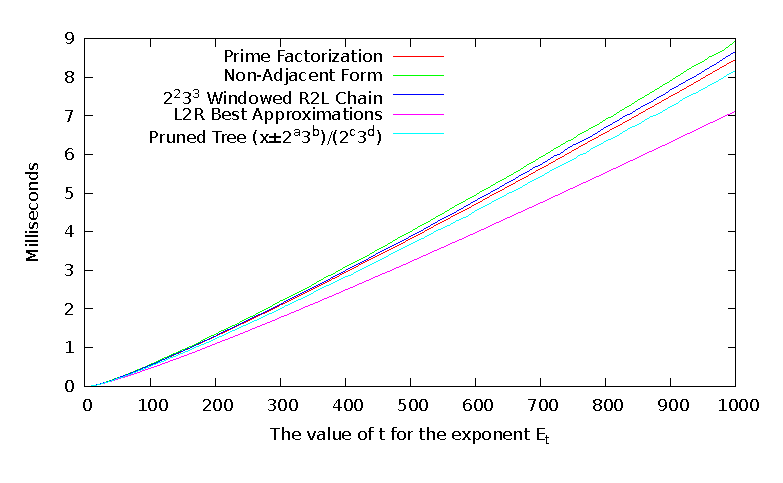
\includegraphics[scale=0.86]{winners-64}
\end{figure}

\end{frame}

% EXPONENTIATION RESULTS (128)
\begin{frame}
\frametitle{Exponentiation Results (128-bit Implementation)}

\begin{figure}
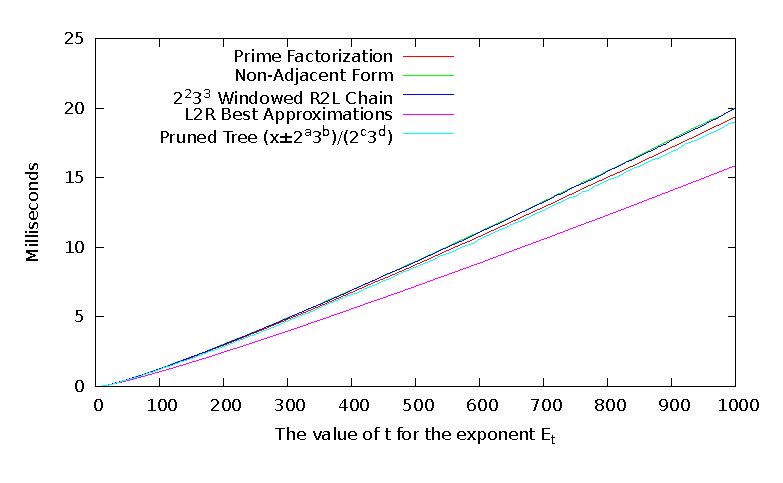
\includegraphics[scale=0.86]{winners-128}
\end{figure}

\end{frame}

% SUPERSPAR
\begin{frame}
\frametitle{SuperSPAR}

SuperSPAR is an integer factoring algorithm based on arithmetic in the ideal class group of imaginary quadratic integers.
\begin{itemize}
\item Extension of SPAR 
\end{itemize}

\end{frame}

\begin{frame}
\frametitle{Factorization of the Order}
\framesubtitle{Example \#1}

$N = 9223375433619660527, k = 1, \Delta = -kN$
\begin{itemize}
\item $\ord(\idealclass{p_{19}}) = 2^2 \cdot 13 \cdot 2770667$
\item $\ord(\idealclass{p_{37}}) = 2^3 \cdot 3 \cdot 13 \cdot 2770667$
\item $\ord(\idealclass{p_{43}}) = 2^4 \cdot 3 \cdot 13 \cdot 2770667$
\item $\ord(\idealclass{p_{47}}) = 2^3 \cdot 3 \cdot 13 \cdot 2770667$
\item $\ord(\idealclass{p_{59}}) = 2^4 \cdot 3 \cdot 13 \cdot 2770667$
\end{itemize}

where $\ideal{p_p} = [p, (b + \sqrt\Delta)/2]$.

\end{frame}

\begin{frame}
\frametitle{Factorization of the Order}
\framesubtitle{Example \#2}

$N = 18278283564428467183, k = 3, \Delta = -4kN$
\begin{itemize}
\item $\ord(\idealclass{p_{11}}) = 2 \cdot 3 \cdot 59 \cdot 157 \cdot 1451$
\item $\ord(\idealclass{p_{17}}) = 2 \cdot 5^2 \cdot 59 \cdot 157 \cdot 1451$
\item $\ord(\idealclass{p_{23}}) = 2 \cdot 3 \cdot 5^2 \cdot 59 \cdot 157 \cdot 1451$
\item $\ord(\idealclass{p_{29}}) = 2 \cdot 3 \cdot 59 \cdot 157 \cdot 1451$
\item $\ord(\idealclass{p_{31}}) = 2 \cdot 5 \cdot 59 \cdot 157 \cdot 1451$

\end{itemize}

where $\ideal{p_p} = [p, (b + \sqrt\Delta)/2]$.

\end{frame}

\begin{frame}
\frametitle{Prime Power Bound}
To 

\end{frame}

\begin{frame}
\frametitle{Reusing the Order}

Once the order of an ideal class is known, we skip the search phase.

\begin{itemize}
\item The exponentiation stage removed all small primes $\Rightarrow$ search stage not necessary.

\item The exponentiation stage did not remove all small primes $\Rightarrow$ stepping coprime will never find the order.
\end{itemize}

For $N \le 2^{80}$, this is expected to work better than 97.7\% of the time.

\end{frame}




% SQUARE ROOT APPROXIMATION
\begin{frame}
\frametitle{Approximate Square Root}
Notice that
\begin{equation*}
\begin{array}{rrlrlr}
	& x^{1/2} &=& 2^{(\log_2x)/2} &\approx& 2^{\floor{\floor{\log_2x+1}/2}} \\
	\Rightarrow & x / x^{1/2} &=& x / 2^{(\log_2x)/2} &\approx& x / 2^{\floor{\floor{\log_2x+1}/2}},
\end{array}
\end{equation*}
which is approximated by shifting $x$ right by $\floor{\floor{\log_2x+1}/2}$ bits.
\end{frame}

% SQRT OPTIMIZATION
\begin{frame}
\frametitle{Square Root Approximation}
\framesubtitle{64-bit Multiplication}
\begin{figure}
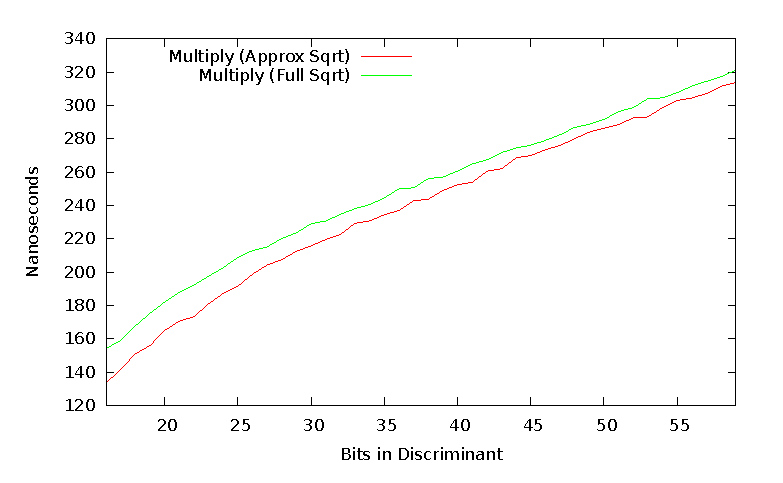
\includegraphics[scale=0.86]{compose-sqrtopt-64}
\end{figure}
\end{frame}

\begin{frame}
\frametitle{Square Root Approximation}
\framesubtitle{128-bit Multiplication}
\begin{figure}
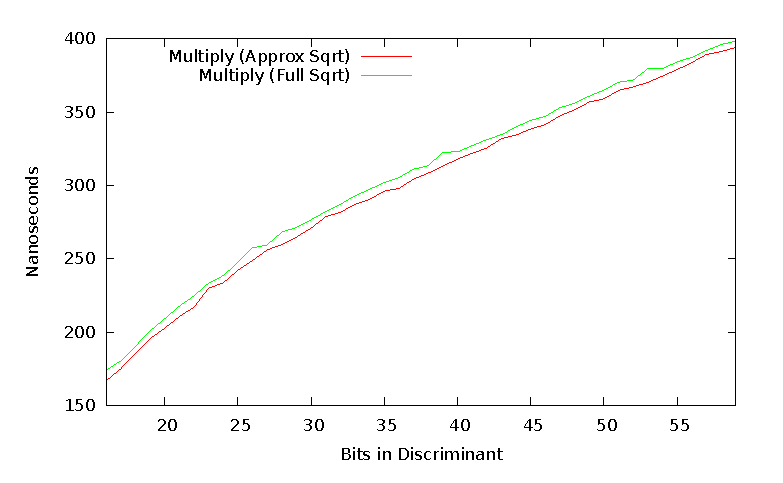
\includegraphics[scale=0.86]{compose-sqrtopt-128}
\end{figure}
\end{frame}

\begin{frame}
\frametitle{Square Root Approximation}
\framesubtitle{64-bit Cubing}
\begin{figure}
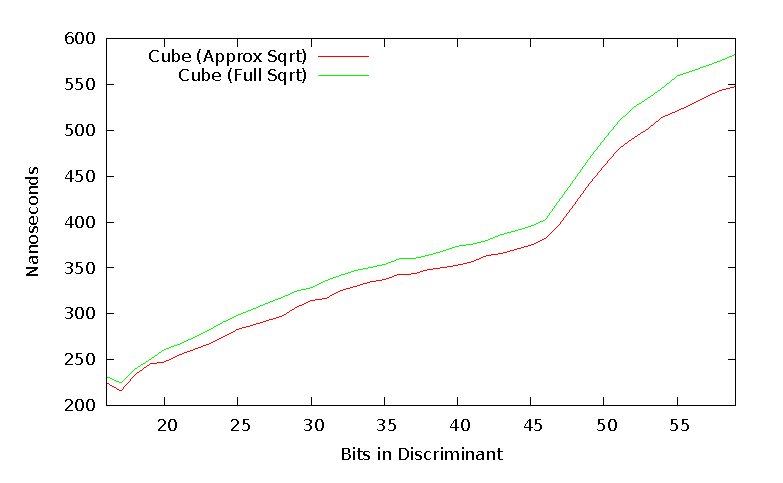
\includegraphics[scale=0.86]{cube-sqrtopt-64}
\end{figure}
\end{frame}

\begin{frame}
\frametitle{Square Root Approximation}
\framesubtitle{128-bit Cubing}
\begin{figure}
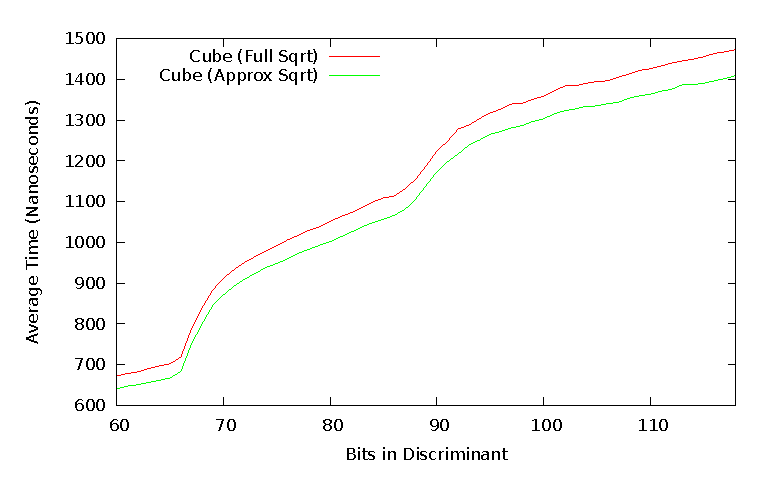
\includegraphics[scale=0.86]{cube-sqrtopt-128}
\end{figure}
\end{frame}




\end{document}

